\scanpage{16}
\handwritten{\mspage{7}}
\margin{\handwritten{\figure{\begin{tikzpicture}[x=1cm,y=1cm]\draw[line width=0.8pt] (0,0.20)--(0.025,0.10)--(0.03,0);\end{tikzpicture}}}}
une nette tendance à être $\handwritten{\ne}0$.

6.\quad \deleted{Conjecture II} \uline{Conjecture}: pour $X$\inserted{$\handwritten{\subset}P^r_k$} fixé\deleted{\unsure{x}}, comme dans 5), \inserted{avec $n\handwritten{\geq}2$,} il existe un entier $d_0$ tel que pour tout pinceau \inserted{de Lefschetz \handwritten{assez général}} de hypersurfaces de degré $d\handwritten{\geq}d_0$ dans $P^r$, donnant une section générique $Y_{\bar s}$ avec $X$, l'inclusion $Y_{\bar s}\handwritten{\hookrightarrow}X_{\bar s}$ satisfait à la condition b) de 2) (le fait que la condition a) doive être vérifiée en tous cas étant de toutes façons justiciable de la conjecture d'algébraicité de la\deleted{opération} correspondance cohomologique $\handwritten{\Lambda}$ sur $X$).
\margin{\handwritten{\figure{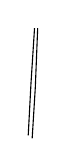
\begin{tikzpicture}[x=1cm,y=1cm]\draw (0.05,0)--(0.09,0.65)--(0.12,1.4);\draw (0,0.04)--(0.035,0.7)--(0.08,1.4);\end{tikzpicture}}}}

Nous allons examiner cette conjecture, en supposant déjà que le \deleted{\unsure{théorè|théoré}} théorème de Lefschetz ``vache'' soit vrai sur $X$, et que la correspondance $\handwritten{\Lambda}$ sur $X$ est algébrique. La théorie des cycles évanescents, qui sera prouvée dans SGA 7 cette année, donne alors ceci: L'orthogonal $E^{2n-1}\handwritten{\unsure{\deleted{(}|\ell}}$ de $H^{2n-1}(X)$, ponsidéré comme plongé dans $H^{2n-1}(Y_{\bar s})$, est un \uline{module simple sous l'action de} $\mathrm{Gal}(k(\bar s)/k(s))$, ainsi que \inserted{\handwritten{sous}} celle de tout sous-groupe \deleted{d'indice fini}\inserted{\handwritten{ouvert}}. (NB pour ce dernier fait, on utilise de façon essentielle qu'on est en dimension impaire $2n-1$, de sorte que les opérations de monodromie locale sont des transvections et non des symétries, \unsure{donc|dont} ne se tuent pas en passant à une puissance quelconque \ldots)Il s'ensuit déjà que \deleted{pour vérifier} la condition b)\deleted{il suffit de vérifier}\inserted{équivaut à dire} que $E^{2n-1}$ \uline{n'est pas tout entier de niveau} 1 . En caractéristique nulle, \deleted{il suffit} s'il était tout entier de niveau 1, \deleted{on en déduirait}\inserted{cela impliquerait} que les composantes de type $p,q$ de $E^{n-1}$ sont nulles sauf les deux composantes $(n,n-1)$ et $(n-1,n)$ (la réciproque étant vraie d'ailleurs si la conjecture de Hodge est vraie); cela \deleted{\unsure{implique que $H$|xxx implique que $H$}} signifie aussi que $\deleted{{\unsure{H|W}}^{\handwritten{2n-1}}(}$ $H^{p,q}(X)\handwritten{\hookrightarrow}H^{p,q}(Y)$ est un isomorphisme pour ces valeurs de $(p,q)$, en particulier que \deleted{il est} $H^{2n-1}(X,\underline{O}_X)\handwritten{\longrightarrow}H^{2n-1}(Y,\underline{O}_Y)$ est un isomorphisme\inserted{\handwritten{(car $n\geq2$)}}, ce qui n'est pas le cas pour $d$ grand (car la dimension du second membre tend vers $\handwritten{\infty}$ avec $d$). Cela prouve (par la méthode de Lefschetz, reprise par Griffiths) l'énoncé voulu en caractéristique nulle.
% archive sheet number: 15
